\documentclass[11pt]{article}
\usepackage[margin=1in]{geometry}
\usepackage{graphicx,booktabs,amsmath,hyperref,array}
\hypersetup{hidelinks}
\title{GLAM against plain pCN on the real tracer problem:\\ the 80\,000-iteration study (s80k)}
\author{Aidan Gettemy}
\date{November 16, 2026}
\begin{document}
\maketitle

\section{Summary}
Six sampling arms were run on the real tracer/Darcy problem (6001-dimensional whitened state: 12 blocks of 500 coefficients and $\rho$), each with 24 chains from random initialisation, 80\,000 iterations and the same fixed step sizes. Arm~1 is plain pCN, the baseline; arms 2--5 are GLAM variants; arm~2b was added during the study. The numbers below come from the returned tables (tail from iteration 40\,000).

\begin{itemize}
\item \textbf{Agreement between chains is not the same as a calibrated posterior.} The unmasked GLAM arms (2, 2b, 3) look converged by R-hat (max PSRF $1.005$--$1.024$) but are too narrow: the $2\sigma$ coverage of the reference field is $0.63$, $0.33$ and $0.74$, against $0.94$ for pCN; the mean posterior sd of $\ln K$ is $0.33$, $0.16$ and $0.43$, against $0.58$.
\item \textbf{Memory (arm 2b) did not speed up the descent beyond arm~2, and it collapsed the spread most.} The $\Phi$ curves of arms 2 and 2b nearly coincide, ending near $780$ (read off the figure) against about $980$ for pCN; 2b has the lowest coverage ($0.33$) and the highest rms $z$-score ($5.48$).
\item \textbf{The keep-own mask restores part of the spread.} Arm~4 against arm~2 and arm~5 against arm~3: $2\sigma$ coverage $0.63\to0.75$ and $0.74\to0.82$, rms $z$ $2.53\to1.87$ and $1.91\to1.53$. The R-hat of the masked arms rises back toward the pCN range (max PSRF $2.85$ and $2.91$ against $3.33$), consistent with the chains no longer being copies of the same anchor in the unconstrained coordinates (not yet checked coordinate by coordinate). Neither masked arm reaches the pCN calibration ($0.94$, $1.07$), and their final $\Phi$ is a little higher than that of their unmasked parents.
\item \textbf{The baseline itself has not converged between chains.} pCN has MPSRF $30.8$ on block~0, max PSRF $3.33$ and no coordinate below $1.1$; $\Phi$ is still falling slowly (about $1100$ at iteration 40\,000, about $980$ at 80\,000). Its pooled field statistics are well calibrated, so it is the best available reference, not ground truth.
\item \textbf{Under these fixed small steps no GLAM variant descends faster than pCN early on}; the six $\Phi$ curves overlap through the first $\approx 10\,000$ iterations (read off the figure). The single-anchor arms end about $20\%$ lower in $\Phi$.
\end{itemize}
Not yet analysed (the data are on the cluster, not in the repository): variance by coefficient index for each arm, the anchor $\Phi$ over exchanges for arms 2, 2b, 3, the leakage check of arms 4--5, and time to a fixed $\Phi$ level.

\section{Design}
\begin{table}[h]\centering\small
\begin{tabular}{@{}llp{9.2cm}@{}}\toprule
arm & tag & what differs \\ \midrule
1 & \texttt{s80k\_pcn} & plain pCN, no exchanges (baseline, and source of the mask) \\
2 & \texttt{s80k\_glam1} & GLAM, one anchor; the pool at an exchange is the chains' current states only; nothing is remembered between exchanges \\
2b & \texttt{s80k\_glam1\_best} & as 2, but the pool also holds the previous anchor and every chain's best state of the stage (elitist: the anchor's $\Phi$ can only fall) \\
3 & \texttt{s80k\_glamN} & many anchors (cap 300, min.\ distance 12, min.\ score 0.5, quality tolerance 400, $\alpha=0.7$), previous anchors and stage-best states in the pool \\
4 & \texttt{s80k\_glam1\_mask} & as 2, with the keep-own mask at every restart \\
5 & \texttt{s80k\_glamN\_mask} & as 3, with the keep-own mask, and distance and log-det selection computed on the constrained coordinates only \\ \bottomrule
\end{tabular}
\caption{The six arms. Common to all: 24 chains, random start, seed 2026, 80\,000 iterations, fixed step sizes $\beta_G=0.011952$, $\beta_L=0.061968$ (the frozen values of earlier runs reduced by 20\%), post-processing tail from iteration 40\,000. In arms 2--5 the anchor exchange is never stopped; GLAM is treated as a population-based optimisation heuristic, not as exact MCMC.}
\end{table}
The keep-own mask (``subspace transplant'') installs the anchor only in the coordinates the data constrain and leaves each chain its own value elsewhere, so that unconstrained directions keep their between-chain variance. The coordinates were chosen from the pooled variance of the pCN chains by index within each block (Section~\ref{sec:mask}); $\rho$ is always taken from the anchor.

\section{Results}
\subsection{Convergence diagnostics}
\begin{table}[h]\centering\small
\resizebox{\textwidth}{!}{% generated by make_fig.py from tables/e6_glam_s80k_*/{mpsrf,field_comparison,diagnostics}.json: do not edit by hand
\begin{tabular}{llrrrrrr}\toprule
arm & & MPSRF $\rho$ & MPSRF first 100 & MPSRF block 0 & PSRF max & PSRF median & coords $<1.1$ \\ \midrule
1 & pCN & 1.341 & 7.279 & 30.82 & 3.329 & 1.974 & 0.00 \\
2 & one anchor & 1.001 & 1.058 & 1.24 & 1.005 & 1.001 & 1.00 \\
2b & one anchor + memory & 1.002 & 1.070 & 1.25 & 1.015 & 1.003 & 1.00 \\
3 & many anchors & 1.008 & 1.104 & 1.34 & 1.024 & 1.009 & 1.00 \\
4 & one anchor + mask & 1.005 & 1.072 & 19.91 & 2.850 & 1.568 & 0.35 \\
5 & many anchors + mask & 1.012 & 1.096 & 21.22 & 2.913 & 1.552 & 0.35 \\
\bottomrule\end{tabular}
}
\caption{MPSRF at the end of the tail and PSRF over all 6001 coordinates. Samples: every 10th iteration from 40\,000 (4000 per chain), 24 chains. The chains of arms 2--5 are coupled through the anchors, so these are mixing diagnostics, not convergence proofs.}
\end{table}
The unmasked GLAM arms have MPSRF close to 1 on $\rho$ and on the first 100 coordinates (convergence below $1.2$ at iteration $\approx 53\,000$--$58\,000$) and just above $1.2$ on block~0; every coordinate has PSRF below $1.1$. Plain pCN does not: its MPSRF is $1.34$ on $\rho$, $7.3$ on the first 100 coordinates and $30.8$ on block~0, and no coordinate has PSRF below $1.1$. The masked arms agree on $\rho$ and on the first 100 coordinates (MPSRF $\le 1.10$) but not on block~0 (MPSRF about $20$) or in the PSRF ($2.85$ and $2.91$; $35\%$ of the coordinates below $1.1$). That is consistent with the chains having regained between-chain variance in some directions; which coordinates, has not been checked.

\subsection{Descent}
\begin{figure}[t]\centering
\begin{tabular}{@{}cc@{}}
\small 1 pCN & \small 2 one anchor \\
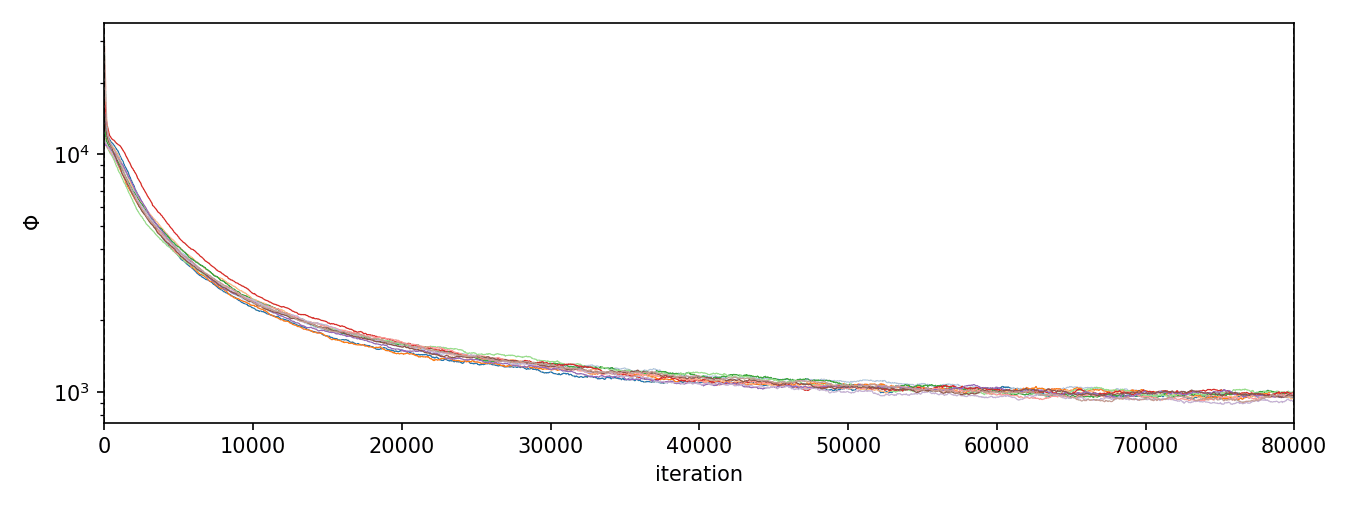
\includegraphics[width=0.49\textwidth]{fig_phi_1.png} & 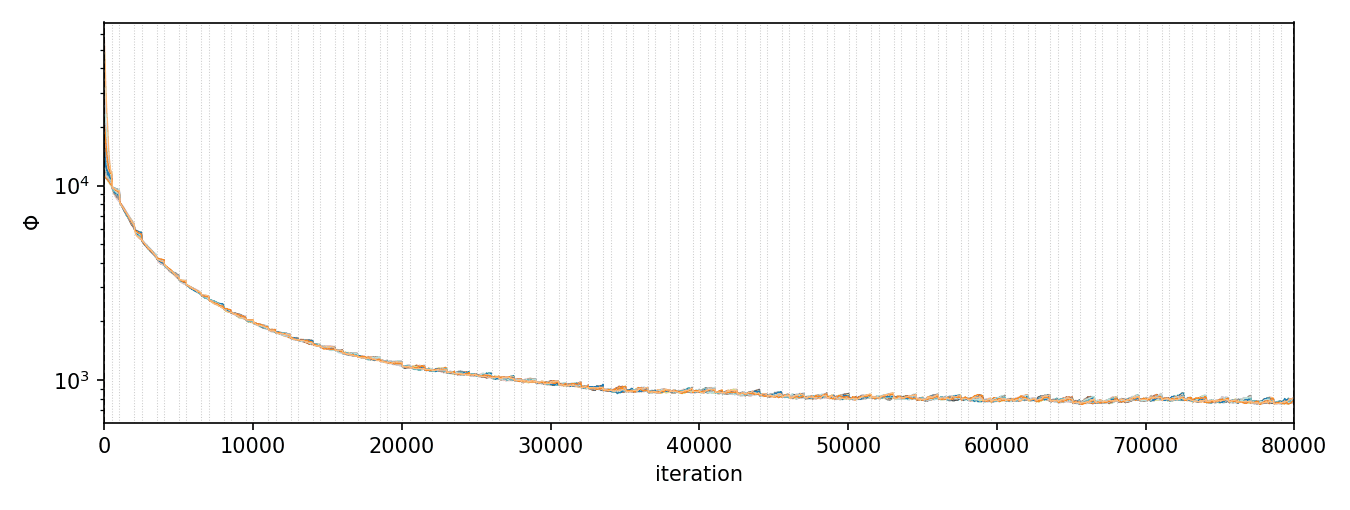
\includegraphics[width=0.49\textwidth]{fig_phi_2.png} \\
\small 2b one anchor + memory & \small 3 many anchors \\
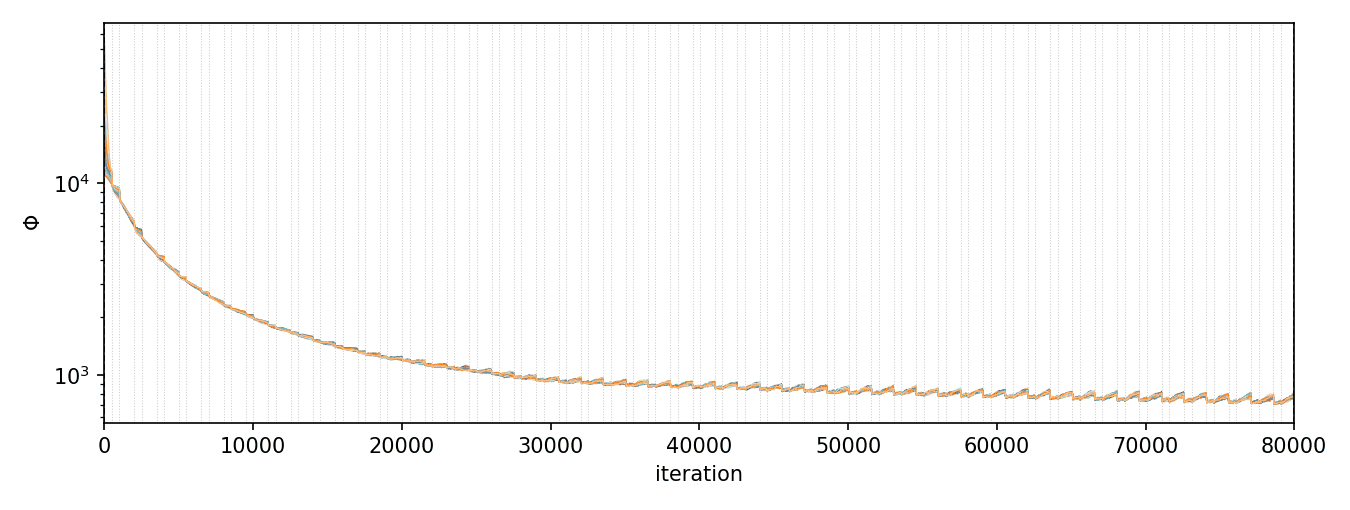
\includegraphics[width=0.49\textwidth]{fig_phi_2b.png} & 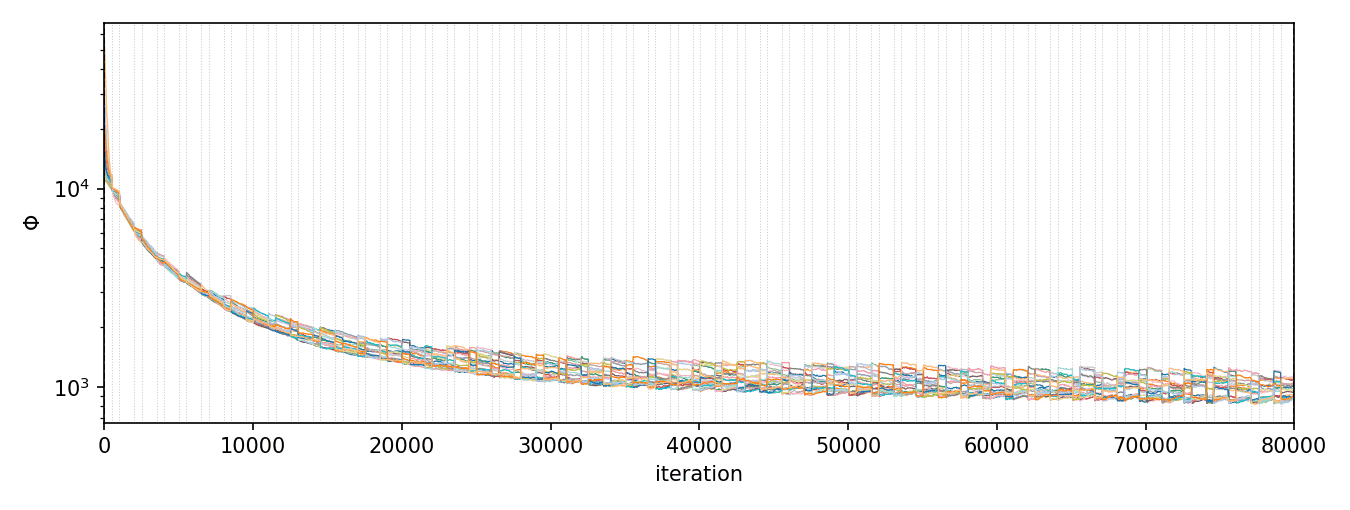
\includegraphics[width=0.49\textwidth]{fig_phi_3.png} \\
\small 4 one anchor + mask & \small 5 many anchors + mask \\
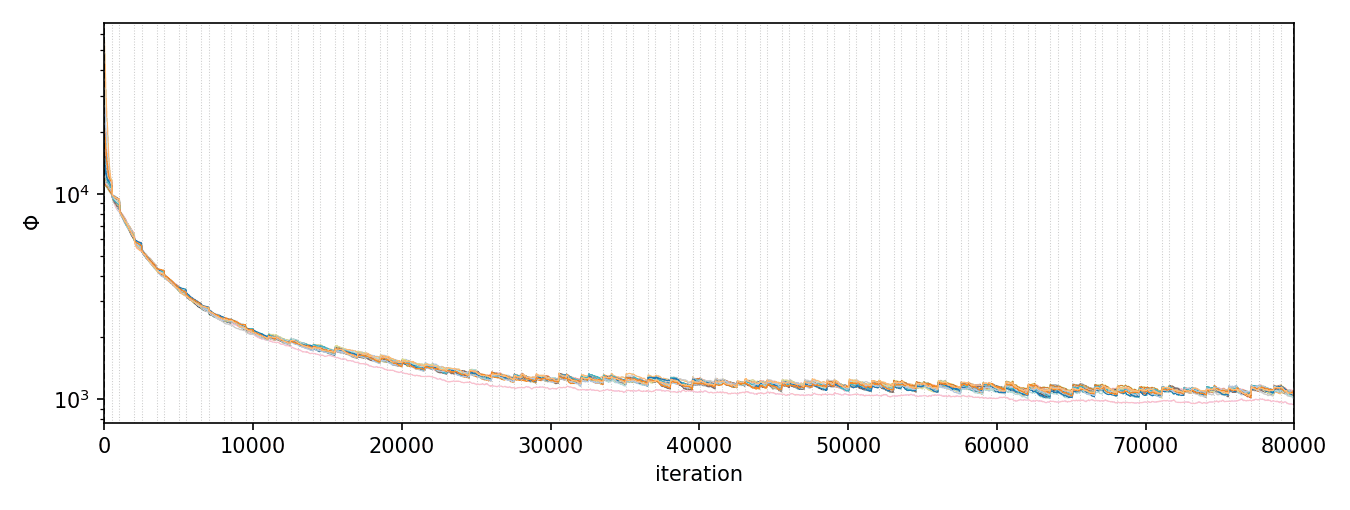
\includegraphics[width=0.49\textwidth]{fig_phi_4.png} & 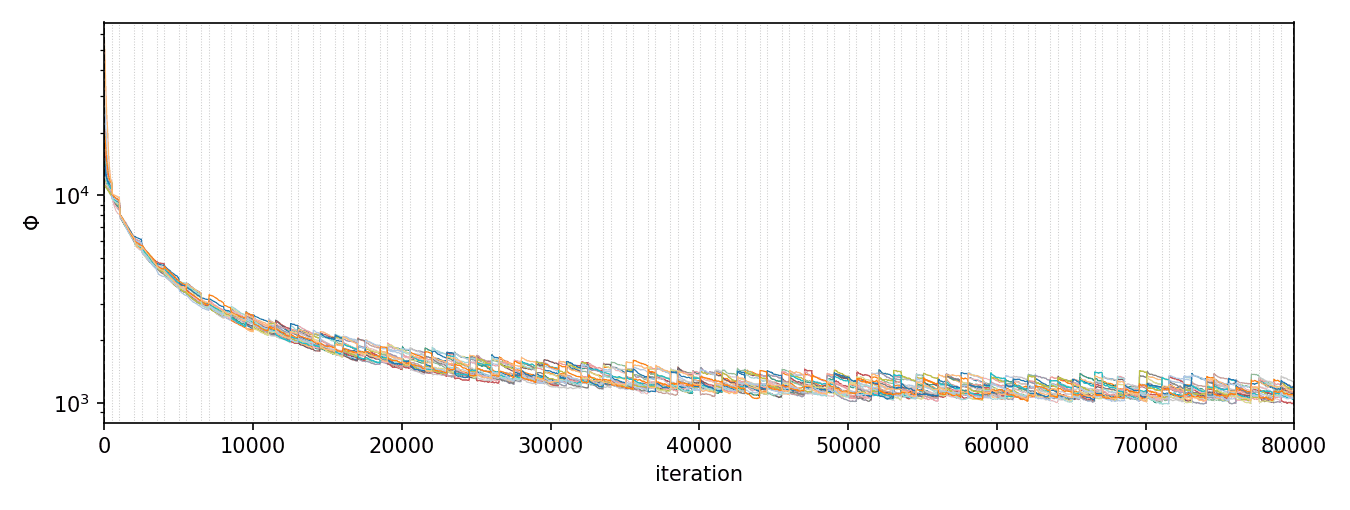
\includegraphics[width=0.49\textwidth]{fig_phi_5.png}
\end{tabular}
\caption{$\Phi$ of all 24 chains against iteration (logarithmic axis). Dotted verticals mark the exchanges. Values quoted in the text are read off these plots.}
\end{figure}
All six arms follow almost the same curve for the first $\approx 10\,000$ iterations ($\Phi\approx 2300$ at iteration 10\,000). From about 15\,000 on the single-anchor arms 2 and 2b bend lower (about $780$ at 80\,000), arm 3 ends near $950$, pCN near $980$, and the masked arms near $1050$--$1100$. The spread of $\Phi$ between chains is smallest in the single-anchor arms, which restart every chain near one state.

\subsection{Calibration against the reference field}
\begin{table}[h]\centering\small
\resizebox{\textwidth}{!}{% generated by make_fig.py: do not edit by hand
\begin{tabular}{llrrrrrr}\toprule
arm & & RMSE of mean & corr.\ of mean & coverage 1$\sigma$ & coverage 2$\sigma$ & rms $z$ & mean sd \\ \midrule
1 & pCN & 0.609 & 0.785 & 0.672 & 0.938 & 1.07 & 0.582 \\
2 & one anchor & 0.707 & 0.699 & 0.353 & 0.626 & 2.53 & 0.325 \\
2b & one anchor + memory & 0.778 & 0.644 & 0.173 & 0.331 & 5.48 & 0.164 \\
3 & many anchors & 0.731 & 0.665 & 0.443 & 0.740 & 1.91 & 0.433 \\
4 & one anchor + mask & 0.721 & 0.675 & 0.442 & 0.745 & 1.86 & 0.417 \\
5 & many anchors + mask & 0.695 & 0.695 & 0.501 & 0.817 & 1.53 & 0.464 \\
\bottomrule\end{tabular}
}
\caption{Posterior mean and sd of $\ln K$ from forward-model samples pooled over the 24 chains (every 100th iteration from 40\,000) against the reference field (sd of the reference $\ln K$: $0.966$). Coverage: fraction of cells whose reference value lies within $1\sigma$ or $2\sigma$ of the posterior mean; rms $z$: root mean square of $(K_{\rm ref}-\text{mean})/\text{sd}$. Ideal values: $0.68$, $0.95$, $1$.}
\end{table}
\begin{figure}[h]\centering
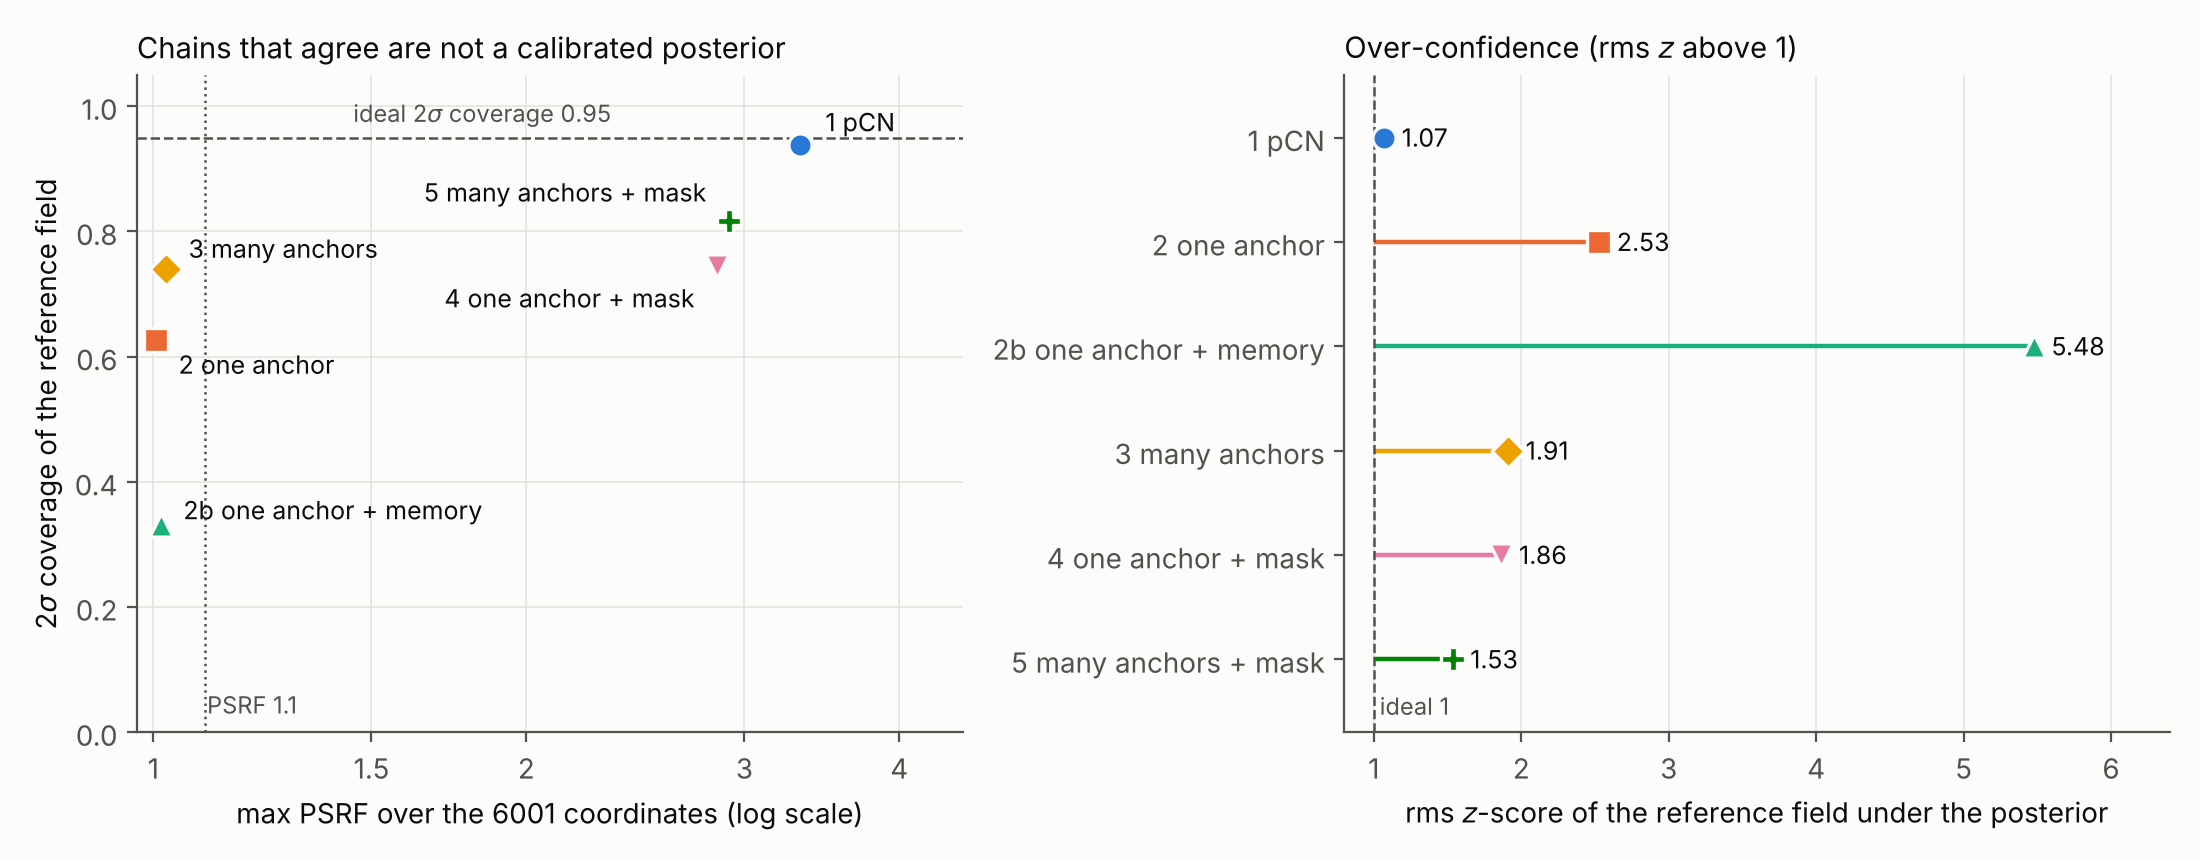
\includegraphics[width=\textwidth]{fig_calibration.png}
\caption{Left: chain agreement (max PSRF, logarithmic axis) against $2\sigma$ coverage; the unmasked GLAM arms sit at PSRF $\approx 1$ and low coverage, pCN at the other extreme. Right: rms $z$-score, lower is better, ideal $1$.}
\end{figure}
pCN is the best calibrated ($0.94$, $1.07$) and also has the smallest error of the posterior mean ($0.609$ against $0.695$--$0.778$ for the GLAM arms). Within the GLAM family the mask helps calibration clearly (arms 4 and 5), while the error of the posterior mean moves little ($0.707\to0.721$ for 2$\to$4, $0.731\to0.695$ for 3$\to$5).

\begin{figure}[h]\centering
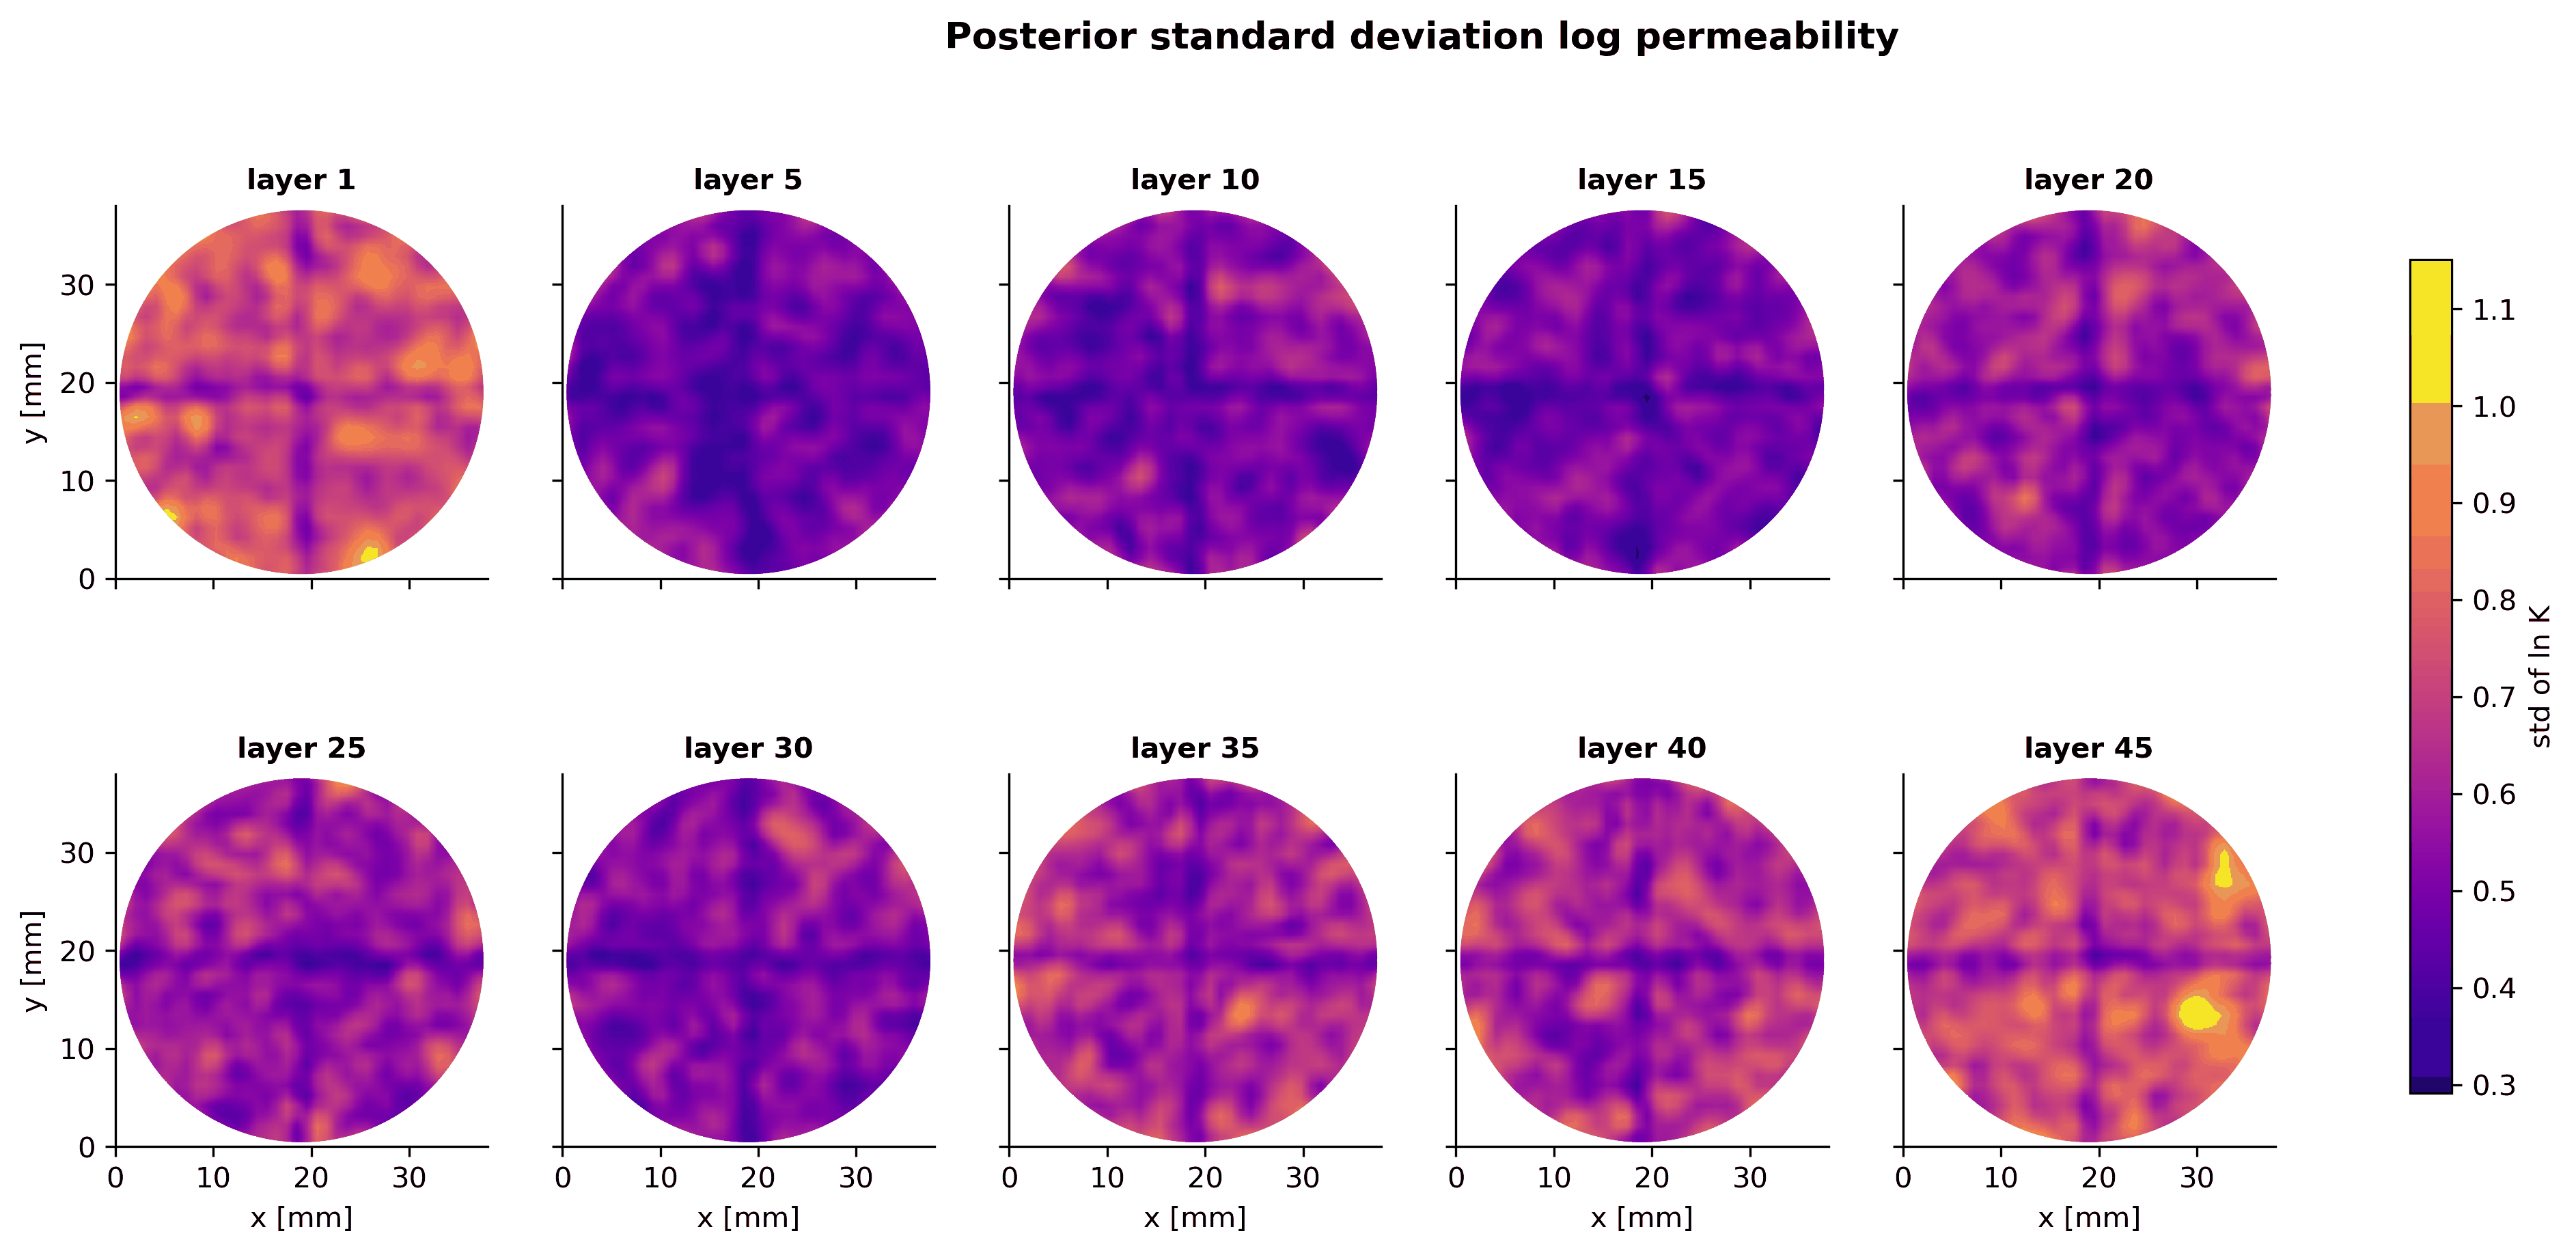
\includegraphics[width=0.82\textwidth]{fig_std_1.png}\\[2pt]
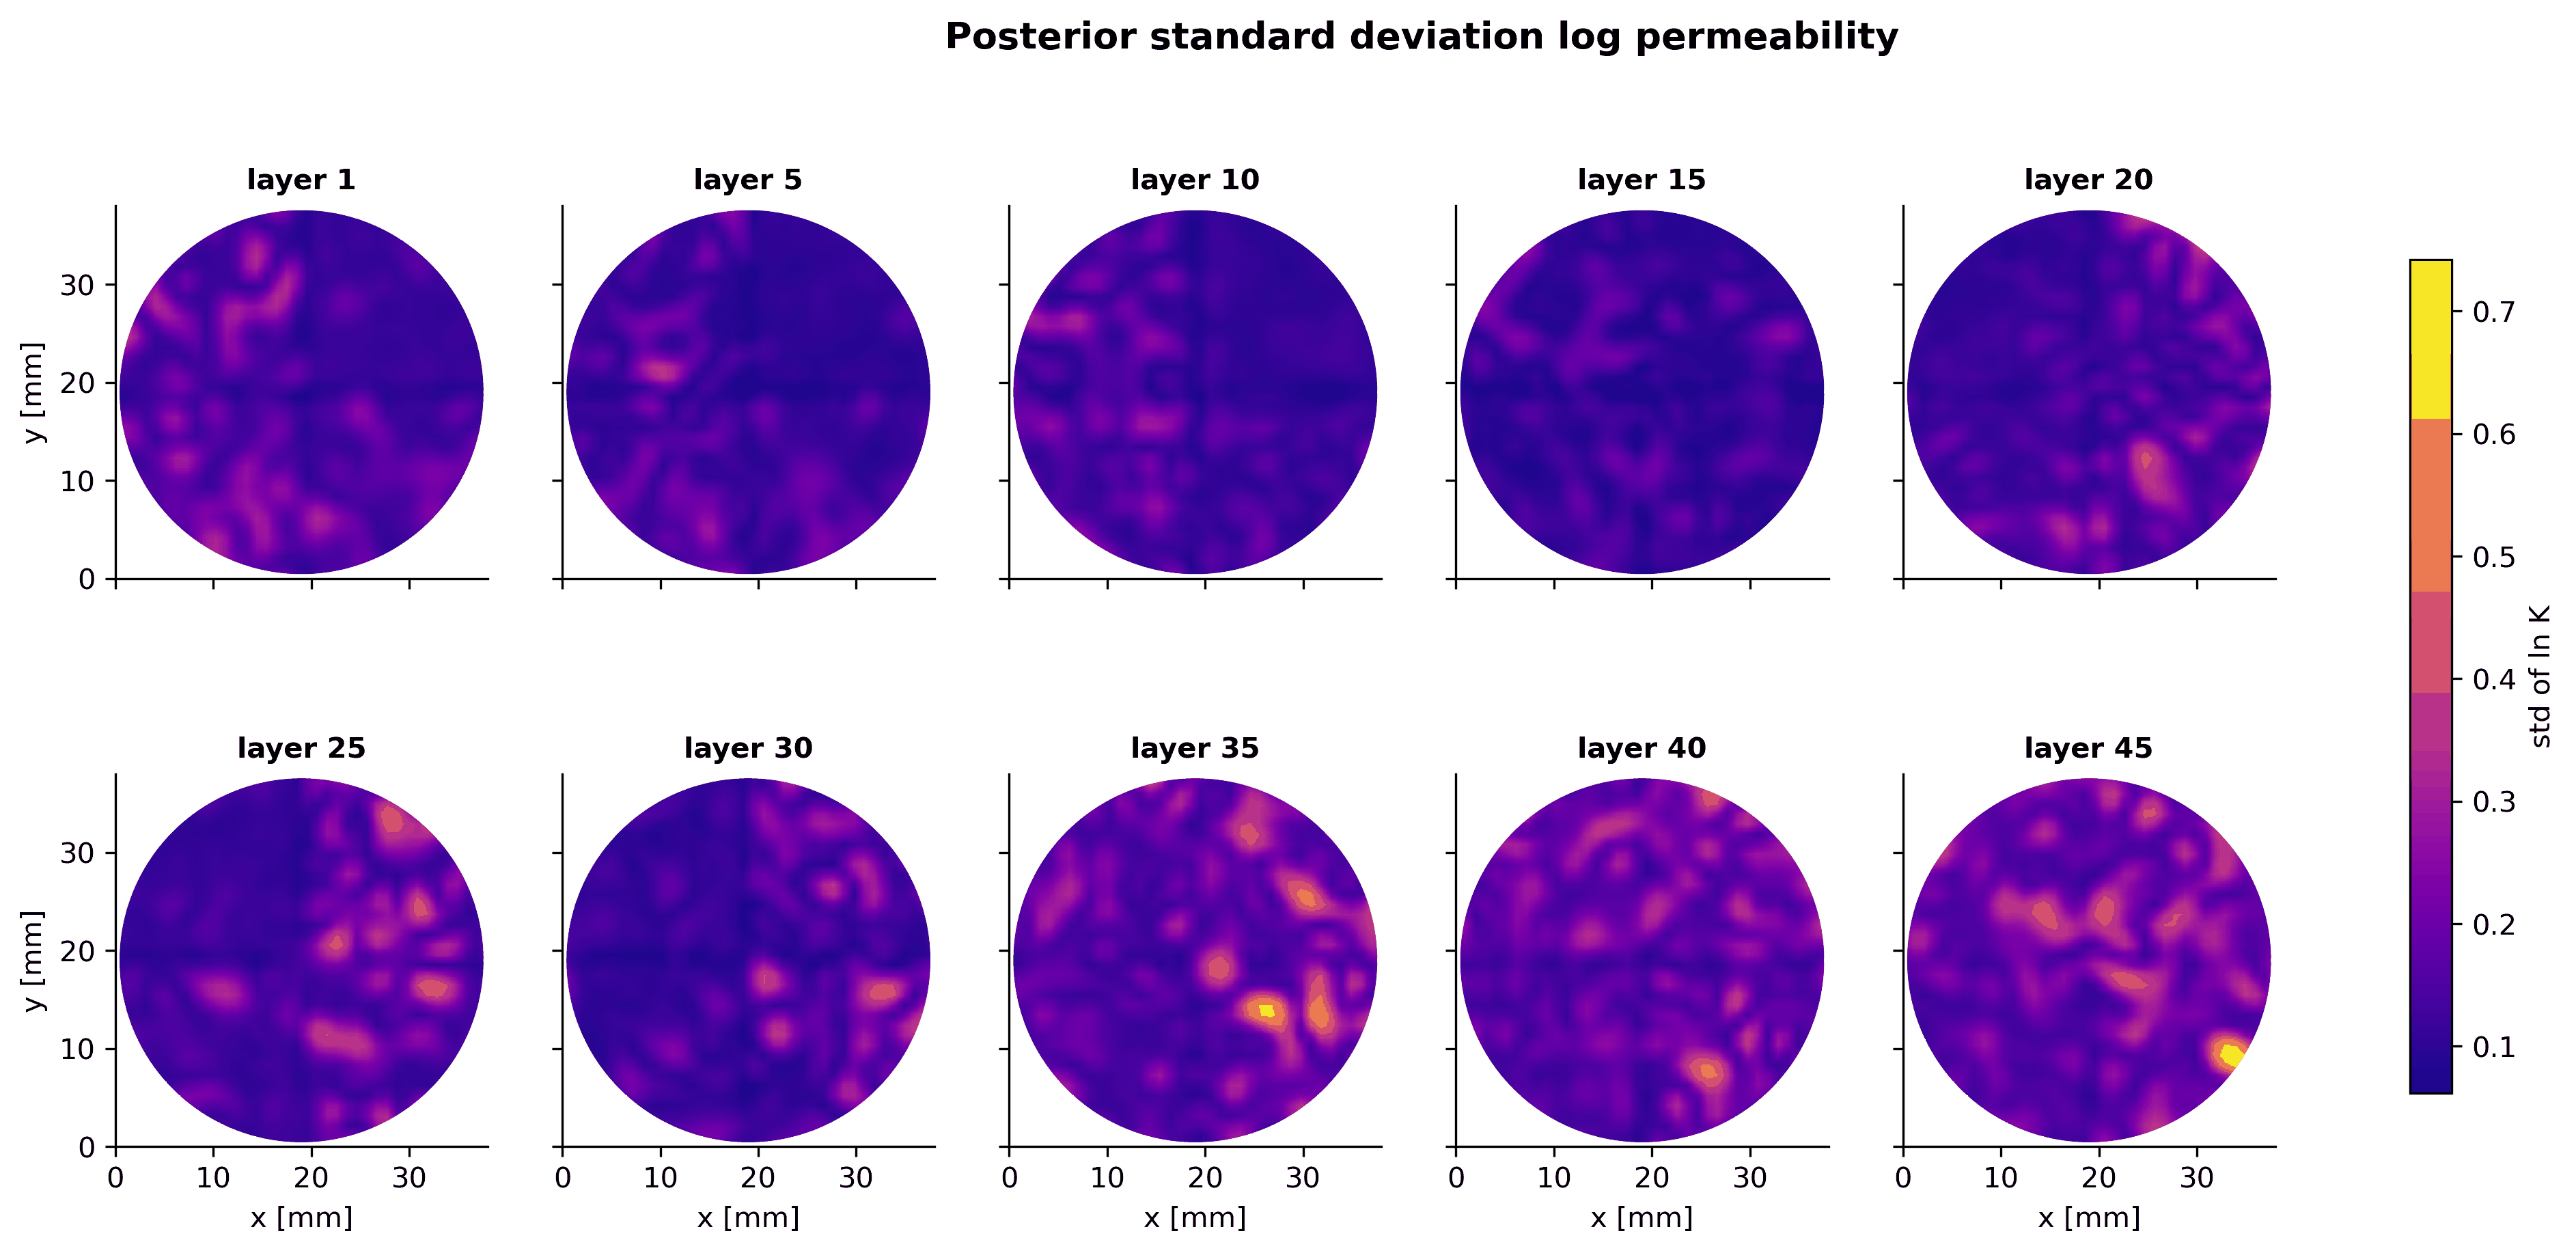
\includegraphics[width=0.82\textwidth]{fig_std_2b.png}\\[2pt]
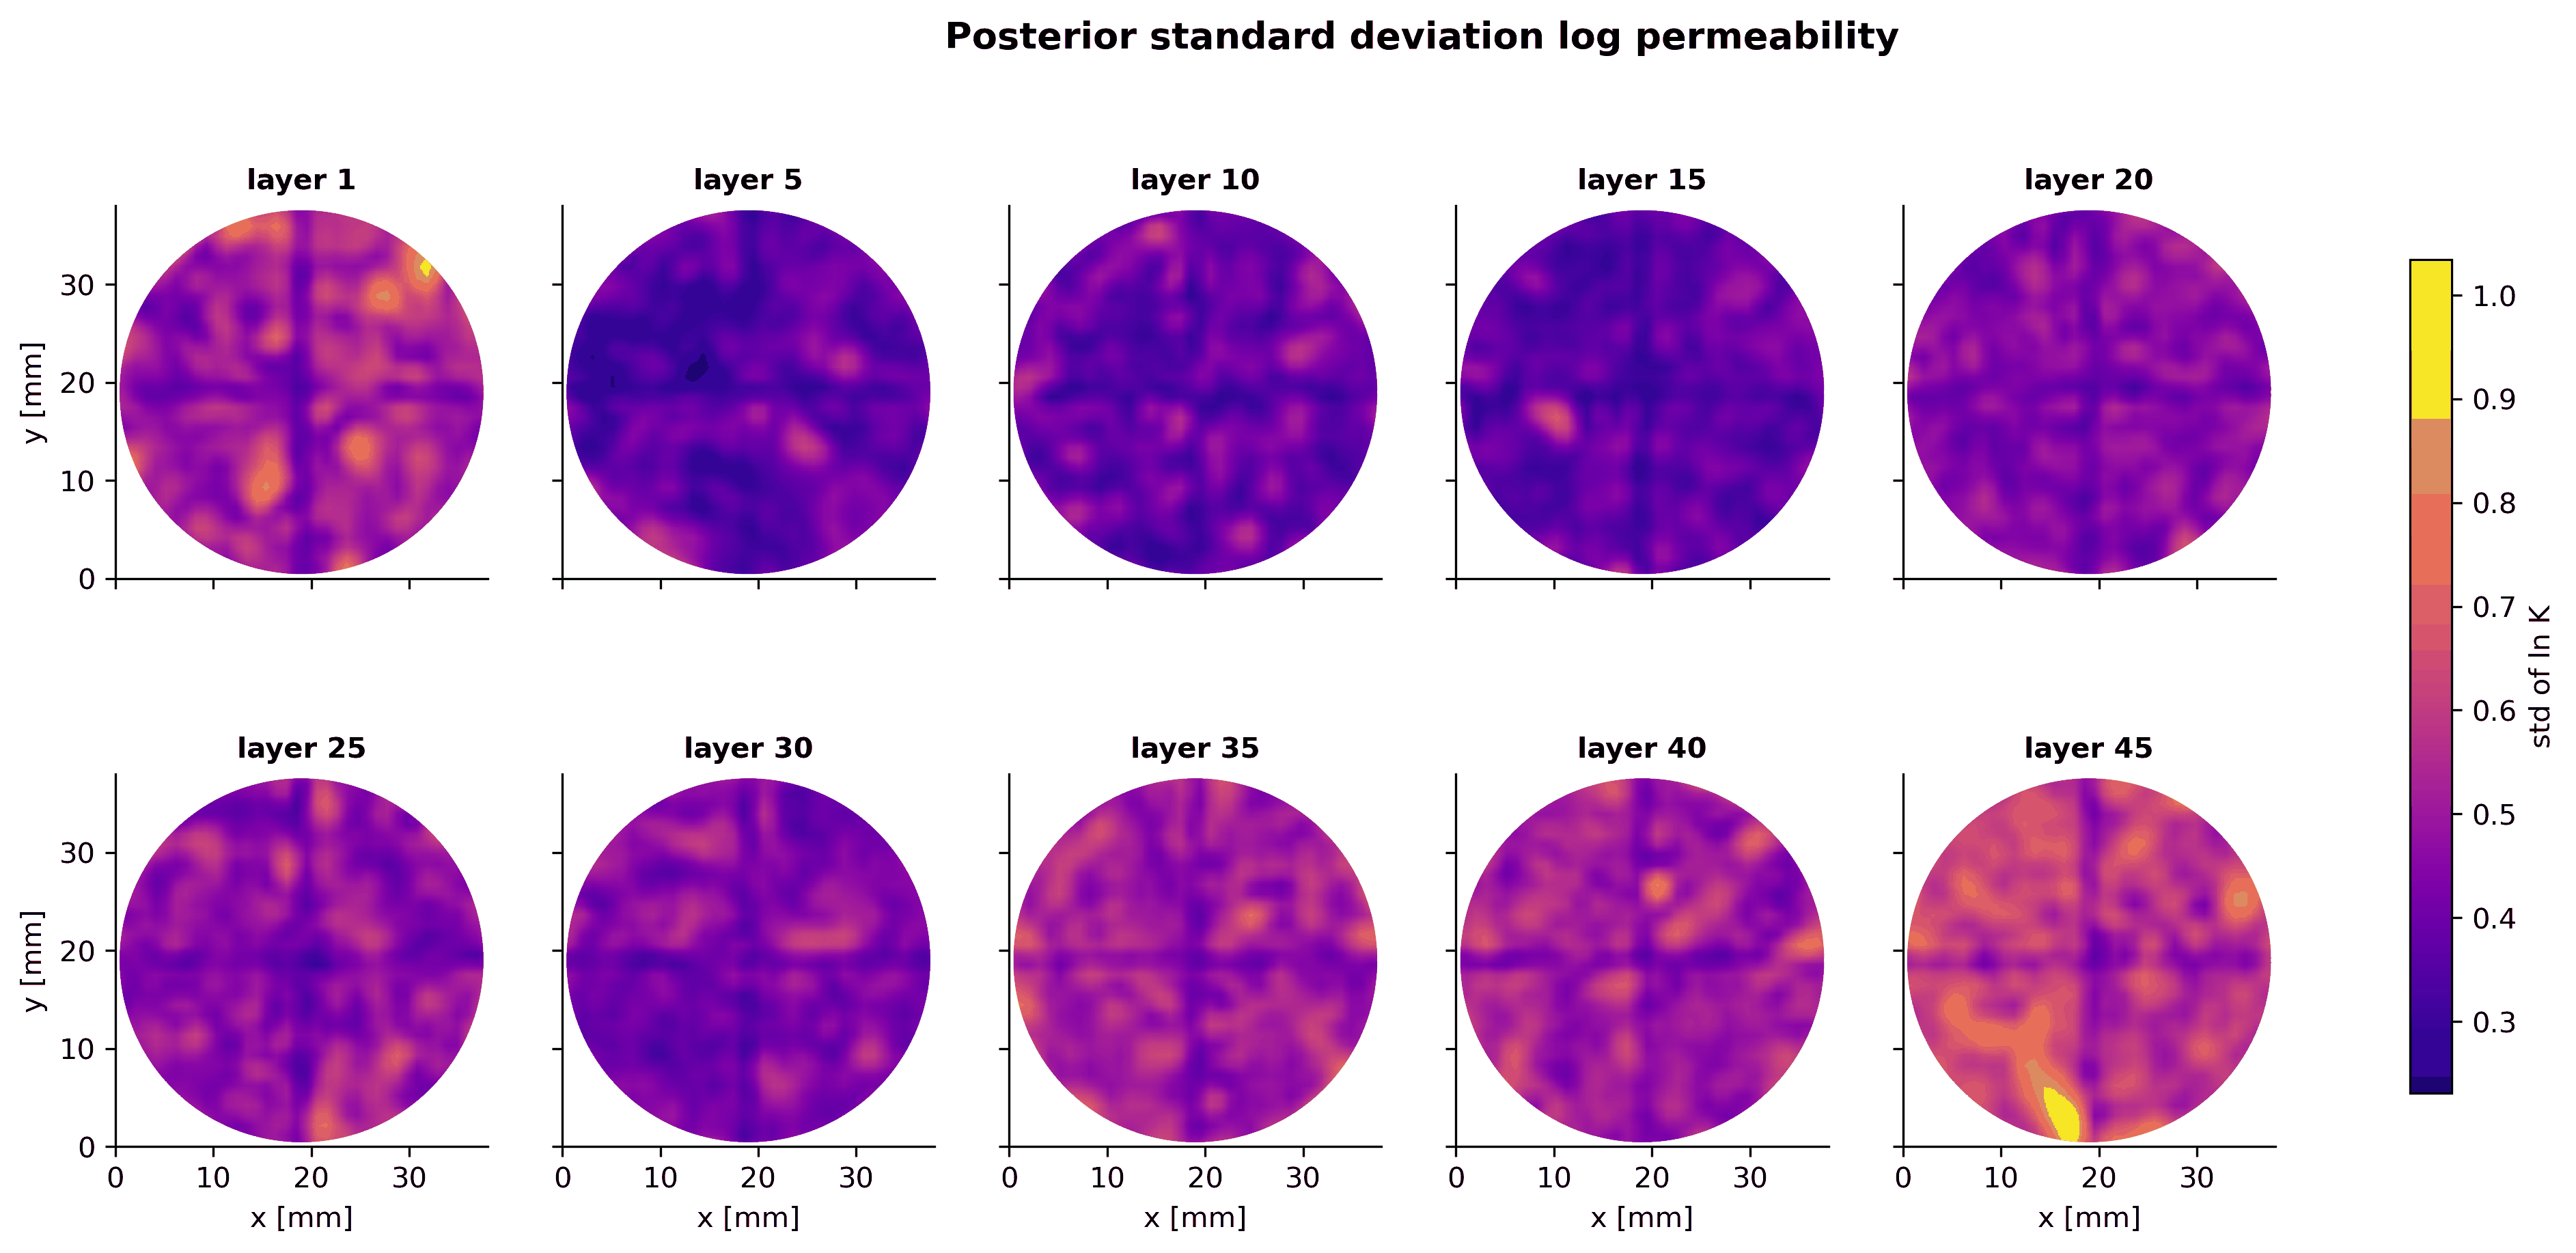
\includegraphics[width=0.82\textwidth]{fig_std_5.png}
\caption{Posterior standard deviation of $\ln K$ in ten layers, for pCN (top), one anchor with memory (middle, note the colour scale ending at $0.7$) and many anchors with the mask (bottom). The figures of the other arms are in \texttt{runs/cluster/figures}.}
\end{figure}

\section{The mask and its sensitivity}\label{sec:mask}
\begin{figure}[h]\centering
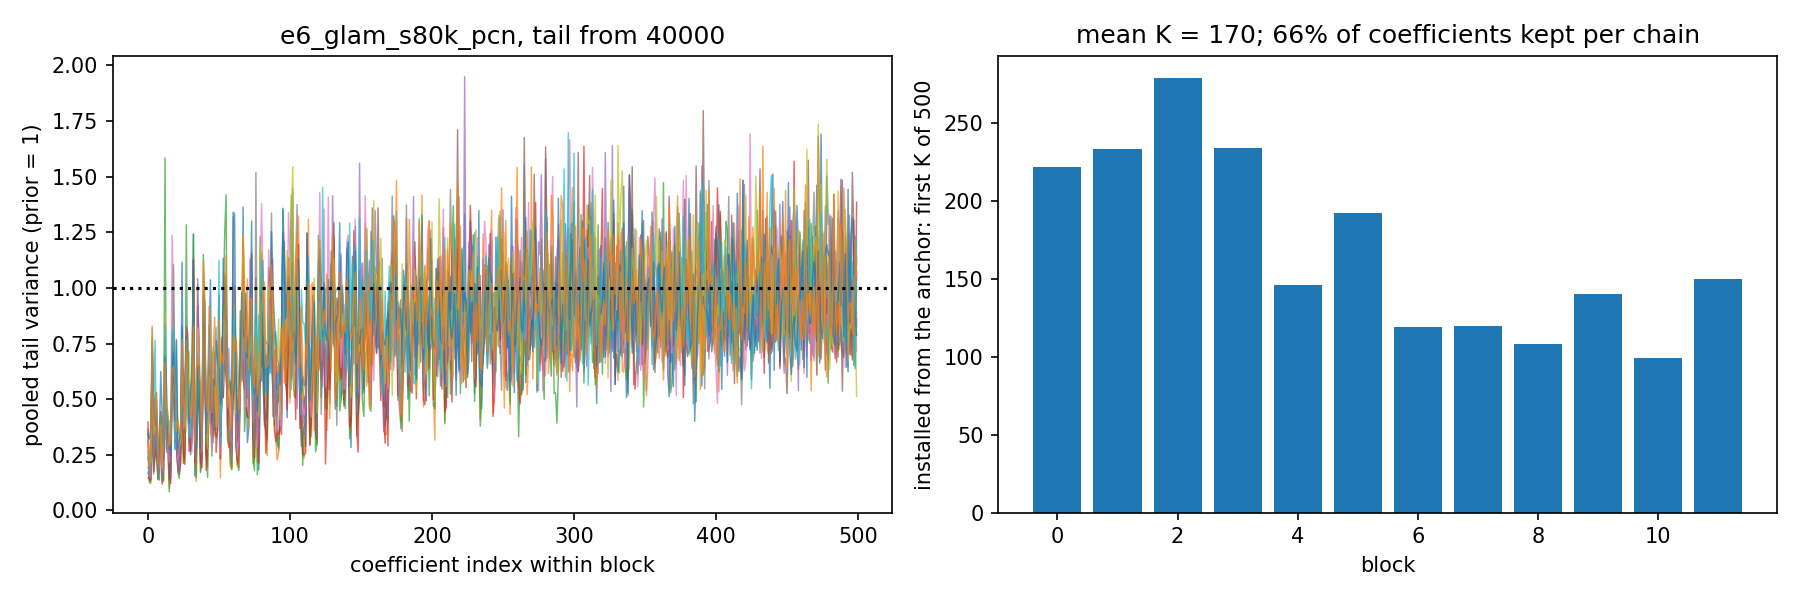
\includegraphics[width=0.95\textwidth]{fig_stage0_24.png}
\caption{Stage 0 on all 24 pCN chains (tail from 40\,000): pooled variance by coefficient index within each block (left; the prior variance is 1) and the number of coefficients installed from the anchor in each block (right). The rise is gradual, there is no sharp elbow; cut-off at smoothed variance $0.8$ plus a margin of $1.5$ (smoothing window 15).}
\end{figure}
\begin{table}[h]\centering\small
\begin{tabular}{@{}lrrrrrrrrrrrrr@{}}\toprule
block & 0&1&2&3&4&5&6&7&8&9&10&11 & total \\ \midrule
12 chains (used by arms 4, 5) & 279&231&279&233&141&149&149&146&105&140&83&174 & 2109 \\
24 chains & 222&233&279&234&146&192&119&120&108&140&99&150 & 2042 \\ \bottomrule
\end{tabular}
\caption{Coefficients installed from the anchor per block (out of 500). Arms 4 and 5 used the mask from the 12 chains that had finished first.}
\end{table}
The total changes by $3\%$, single blocks by up to $57$ coefficients ($20\%$ for block~0). Because the variance rises slowly, a small change of the estimate moves the crossing point by tens of indices. The 12-chain mask was therefore a reasonable estimate, and the difference between the two gives a rough size for its uncertainty.

\section{Incident: the pCN chains that stalled}
In the first run 12 of the 24 pCN chains stopped writing at 5\,500--27\,500 iterations while the other 12 finished, and several resumes wrote nothing. Two defects were found and fixed (merged to \texttt{main}): (i) the chain writer did \texttt{reshape(0,-1)} on an empty record list, which NumPy rejects, so a chain with no accepted move in a 500-iteration window died at its next snapshot and its rank then waited in \texttt{MPI\_Finalize} at 100\% CPU while the job continued silently (the original crash trace was not seen; the resumed run showed the same traceback); (ii) on a resume, ranks whose chains were already finished never called the tracer, whose lazy \texttt{petsc4py} import is collective, so the other ranks hung inside that import. After the fixes the 12 chains advanced at roughly 7\,000--8\,000 iterations per hour (estimated from snapshot times) and finished. \texttt{run\_glam.py} now aborts all ranks on an exception. Arm~1's chains are therefore partly resumed from snapshots (state, random-number state and step sizes restored; at most 500 iterations lost per chain).

\section{Limitations}
\begin{itemize}
\item One seed per arm; no estimate of run-to-run variability. Differences of the size of the arm 4/arm 2 comparison should be treated as indications.
\item Fixed step sizes (the frozen values of earlier runs minus 20\%); GLAM's own adaptation was not exercised.
\item Exchanges were never stopped, so arms 2--5 are not exact MCMC; PSRF and MPSRF of coupled chains are mixing diagnostics.
\item The baseline has not converged between chains at 80\,000 iterations, and the mask was estimated from chains that had not converged in the unconstrained directions.
\item Calibration is measured against a single synthetic reference field.
\item Quantities that need the chains or the exchange summaries (variance by index per arm, anchor $\Phi$, leakage, time to a fixed $\Phi$) are not in this report because those files stay on the cluster.
\end{itemize}

\section{Next steps}
\begin{enumerate}
\item Return exchange summaries and run the variance-by-index analysis on arms 2, 2b, 3, 4, 5 to see whether the remaining shortfall of the masked arms sits in the constrained or in the unconstrained coordinates.
\item Check the leakage of arms 4 and 5 (the $\Phi$ of a transplanted state against its anchor); widen the mask (threshold $0.9$, 3014 coordinates) if it is large.
\item A second seed for arms 3 and 5, and optionally a masked arm 2b.
\item Decide, with the group, how to frame GLAM: as an optimiser (arms 2 and 2b reach lower $\Phi$) or as a sampler (calibration is still below pCN).
\end{enumerate}

\appendix
\section{How the numbers are computed}
\textbf{MPSRF} (Brooks--Gelman, the group's MATLAB convention, \path{brho/mpsrf.py}) for $m=24$ chains and $n$ samples per window, with $W$ the mean within-chain covariance and $B/n$ the covariance of the chain means:
\[
\mathrm{MPSRF}=\sqrt{\tfrac{n-1}{n}+\tfrac{m+1}{m}\,\lambda_{\max}\!\big(W^{-1}B/n\big)} .
\]
Samples are every 10th iteration from 40\,000. ``$\rho$'' is the whitened $\rho$ coordinate, ``first 100'' the first 100 coordinates and ``block 0'' the 500 coefficients of block~0.

\textbf{PSRF} per coordinate is $\sqrt{V_{ii}/W_{ii}}$ with $V=\tfrac{n-1}{n}W+\tfrac{m+1}{m}\tfrac Bn$; the tables give the maximum and the median over all 6001 coordinates.

\textbf{Source tables:} the folders \path{runs/cluster/tables/e6_glam_s80k_pcn}, \path{..._glam1}, \path{..._glam1_best}, \path{..._glamN}, \path{..._glam1_mask} and \path{..._glamN_mask}, files \path{mpsrf.json}, \path{field_comparison.json} and \path{diagnostics.json}. The tables and figures of this report are produced by \path{reports/glam_study80k/make_fig.py}.
\end{document}
